% questions.tex —— 1977 年·江苏南京市初试卷 · 题目内容片段（无答案）
% 由 tools/generate_projects.py 依来源总账自 1977/1977_数学真题_江苏南京市初试_试题.md 生成，勿手改（改源 MD 后重跑）


\gkpart{江苏南京市初试卷}

\begin{gktip}
\textbf{来源说明}：本卷为 1977 年高校招生南京市初试（预选）数学试卷，依据固定源 PDF 第 1—2 页逐题转录。源 PDF 为汇编材料扫描件，第 1 页页首印有分节标题「一、南京市」（H1 按原卷逐字转写，「南 京 市」三字原卷间有排版空隙），同页左下角印有原书页码 230，第 2 页无页码。原卷大题号用中文数字「一、……十、」，本库转写为「\textbf{N．}」；题一、二、四的小题原卷用阿拉伯数字「1．2．…」编号，题十用「①②③」编号，本库统一转写为「（N）」。原卷无分值标注，无附加题与参考题。源卷为纯题面扫描，未附答案；配套答案与解析为本库编者独立推导，\textbf{非官方标准答案}。
\end{gktip}

\par\medskip

\begin{question}
\gkti{1}写出下列各题的正确结果：

（1） $\sqrt{\left(\sqrt{2}-\sqrt{3}\right)^{2}}$；

（2） $0.2^{7}\times5^{7}$；

（3） $\log_{3}27^{-1}$；

（4） $\operatorname{tg}10^{\circ}\operatorname{tg}20^{\circ}\operatorname{tg}70^{\circ}\operatorname{tg}80^{\circ}$。

\end{question}
\begin{question}
\gkti{2}用“$<$”或“$>$”符号把下列各组的值连结起来：

（1） $\log_{2}\dfrac{3.14}{\pi}$ 与 $0$；

（2） $\cos40^{\circ}$ 与 $\sin40^{\circ}$；

（3） $\left(\dfrac{2}{5}\right)^{-\frac{2}{3}}$ 与 $\left(\dfrac{2}{5}\right)^{-\frac{1}{2}}$；

（4） $0.\dot{3}$ 与 $\dfrac{3}{10}$。

\end{question}
\begin{question}
\gkti{3}求 $\sin165^{\circ}$ 与 $\cos255^{\circ}$ 的值。

\end{question}
\begin{question}
\gkti{4}求极限值：

\Needspace{5\baselineskip}
（1） 

\nopagebreak[4]
\[
\lim_{x\to2}\frac{2x^{2}-3x-2}{x-2}\text{\text{；}}
\]

\Needspace{5\baselineskip}
（2） 

\nopagebreak[4]
\[
\lim_{x\to\infty}\frac{3x^{2}-4x+5}{2x^{2}+x-1}\text{。}
\]

\end{question}
\begin{question}
\gkti{5}解方程组

\nopagebreak[4]
\[
\begin{cases}
\dfrac{3x-5y}{2xy}=1\dfrac{1}{3}\\[8pt]
\dfrac{3}{x}+\dfrac{1}{y}=4
\end{cases}
\]

\Needspace{0.4\textheight}
\end{question}
\begin{question}
\gkti{6}在 $\odot O$ 中，直径 $AB$ 和弦 $AC$ 的夹角为 $15^{\circ}$，过 $C$ 点的切线和 $AB$ 的延长线相交于 $P$，已知 $OP=24\,\mathrm{cm}$，求 $\odot O$ 的半径。

\begin{gktip}
原源 PDF 第 2 页附有圆与切线的示意图；LaTeX 版按源图重绘。
\end{gktip}
\nopagebreak[4]
\begin{center}% 1977 年江苏南京市初试卷第六题：圆 O 中直径 AB 与弦 AC 的夹角 15°，过 C 的切线交 AB 延长线于 P，OP=24cm（按源卷第 2 页布局；r=2，OP=2/\cos30°≈2.309，P 在 B 右侧）
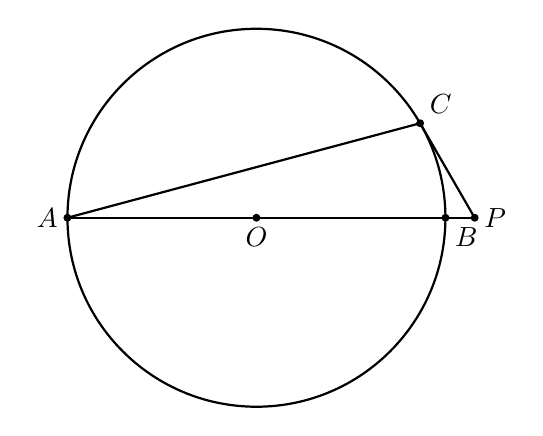
\begin{tikzpicture}[scale=1.2]
  \coordinate (O) at (0,0);
  \coordinate (A) at (-2,0);
  \coordinate (B) at (2,0);
  \coordinate (C) at (1.732,1);
  \coordinate (P) at (2.309,0);
  \draw[thick] (O) circle (2);
  \draw[thick] (A)--(P);
  \draw[thick] (A)--(C);
  \draw[thick] (C)--(P);
  \fill (O) circle (1.2pt) node[below] {$O$};
  \fill (A) circle (1.2pt) node[left] {$A$};
  \fill (B) circle (1.2pt) node[below right] {$B$};
  \fill (C) circle (1.2pt) node[above right] {$C$};
  \fill (P) circle (1.2pt) node[right] {$P$};
\end{tikzpicture}
\end{center}
\nopagebreak[4]
\end{question}
\begin{question}
\gkti{7}设直线 $l_{1}$ 和 $l_{2}$ 的斜率是方程 $6x^{2}-x-1=0$ 的两个根，求直线 $l_{1}$ 和 $l_{2}$ 的交角。

\end{question}
\begin{question}
\gkti{8}把极坐标方程 $\rho=4\sin\theta$ 化为直角坐标方程。

\end{question}
\begin{question}
\gkti{9}甲乙两地相距 12 公里，一货船由甲地顺流航行到乙地装货，返航时每小时速度减少了 4 公里，因此比去时多用了 30 分钟，求该船去时速度。

\end{question}
\begin{question}
\gkti{10}在 $\triangle ABC$ 中，$\angle A$ 的正切是 2，$\angle B$ 的正切是 3，

（1） 求 $\angle C$ 的正切；

（2） 这个三角形是钝角三角形、锐角三角形、还是直角三角形？为什么？

（3） 设这个三角形最短边是 1，求它的最长边。

\end{question}